\documentclass[brazil,aspectratio=169]{lapesd-slides}

\usepackage{booktabs}
\usepackage{colortbl}
\usepackage{tikz}
\usetikzlibrary{positioning}

\graphicspath{ {./images/} }

%%%%%%%%%%%%%%%%%%%%%%%%%%%%
% Metadados
%%%%%%%%%%%%%%%%%%%%%%%%%%%%

\title[]{Soluções para a Convergência entre Computação de Alto Desempenho e Computação em Nuvem}
\author[Artur Luiz Rizzato Toru Soda]{Artur Luiz Rizzato Toru Soda\inst{1} \\ {\small Orientador: Prof. Dr. Márcio Castro\inst{1}}}

\institute{
    \fontsize{10.5}{12.6}\selectfont
        \textit{Distributed Systems Research Lab} -- LaPeSD\\
        Depto. de Informática e Estatística\\
        Universidade Federal de Santa Catarina -- Florianópolis
}

\date{SIC UFSC 2026}

%%%%%%%%%%%%%%%%%%%%%%%%%%%%
% Slides
%%%%%%%%%%%%%%%%%%%%%%%%%%%%

\begin{document}

\titleframe

\begin{frame}{Sumário}
    \tableofcontents
\end{frame}

%%%%%%%%%%%%%%%%%%%%%%%%%%%%
\showsections
\section{Motivação}
%%%%%%%%%%%%%%%%%%%%%%%%%%%%

\begin{frame}{Computação de Alto Desempenho na Nuvem}
    \begin{columns}
        \begin{column}{0.55\textwidth}
            \begin{itemize}
                \item Aplicações científicas exigem grande poder computacional
                \vspace{0.5em}
                \item Provedores de nuvem como a AWS oferecem recursos computacionais sob demanda, sem infraestrutura própria
                \vspace{0.5em}
                \item \textbf{Instâncias \textit{spot}:} capacidade ociosa da AWS com descontos de até 90\%
                \vspace{0.5em}
                \item Preços muito atrativos, porém com uma desvantagem importante
            \end{itemize}
        \end{column}
        \begin{column}{0.42\textwidth}
            \centering
            
\includegraphics[width=0.85\linewidth]{HPConCloud}
        \end{column}
    \end{columns}
\end{frame}

\begin{frame}{O Problema das Instâncias \textit{Spot}}
    \begin{columns}
        \begin{column}{0.55\textwidth}
            \begin{itemize}
                \item \textbf{Instâncias \textit{spot}} podem ser encerradas a qualquer momento, com aviso prévio de apenas \textbf{2 minutos}
                \vspace{0.8em}
                \item \textbf{Aplicações MPI} distribuem a computação entre múltiplos nós de forma \textbf{fortemente acoplada:}
                \begin{itemize}
                    \vspace{0.3em}
                    \item A falha de \textbf{um único nó} encerra toda a execução
                    \vspace{0.3em}
                    \item \textbf{Horas de processamento acumulado se perdem por completo}
                \end{itemize}
            \end{itemize}
        \end{column}
        \begin{column}{0.42\textwidth}
            \centering
            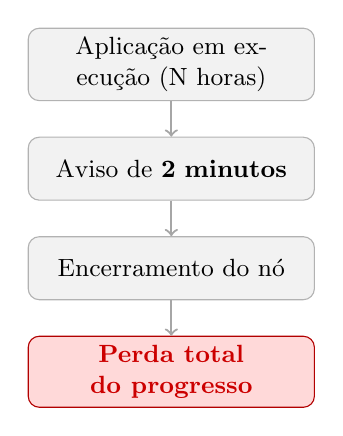
\begin{tikzpicture}[
                node distance=0.45cm,
                box/.style={draw=gray!60, rounded corners=4pt, fill=gray!10,
                            text width=3.4cm, align=center,
                            minimum height=0.8cm, font=\small},
                redbox/.style={draw=red!70!black, rounded corners=4pt, fill=red!15,
                               text width=3.4cm, align=center,
                               minimum height=0.8cm, font=\small\bfseries,
                               text=red!80!black},
                arr/.style={->, thick, gray!70}
            ]
                \node[box] (job) {Aplicação em execução (N horas)};
                \node[box, below=of job] (warn) {Aviso de \textbf{2 minutos}};
                \node[box, below=of warn] (term) {Encerramento do nó};
                \node[redbox, below=of term] (loss) {Perda total do progresso};
                \draw[arr] (job) -- (warn);
                \draw[arr] (warn) -- (term);
                \draw[arr] (term) -- (loss);
            \end{tikzpicture}
        \end{column}
    \end{columns}
\end{frame}

\begin{frame}{Checkpoint/Restart: a Solução Clássica}
    \begin{columns}
        \begin{column}{0.52\textwidth}
            \textbf{Como funciona:}
            \begin{itemize}
                \item Salvar periodicamente o estado completo da aplicação em armazenamento persistente
                \vspace{0.4em}
                \item Em caso de falha, retomar a execução do ponto salvo sem reiniciar do zero
                \vspace{0.4em}
                \item Amplamente adotado em HPC para tolerar interrupções
            \end{itemize}
        \end{column}
        \begin{column}{0.45\textwidth}
            \begin{alertblock}{Limitações das soluções atuais}
                \small
                \begin{itemize}
                    \item Exigem \textbf{modificações no código fonte}, inviabilizando aplicações MPI legadas
                    \vspace{0.3em}
                    \item Dependem de \textbf{identidades de rede fixas} (IPs e hostnames imutáveis), condição que instâncias \textit{spot} não garantem
                \end{itemize}
            \end{alertblock}
        \end{column}
    \end{columns}
\end{frame}

%%%%%%%%%%%%%%%%%%%%%%%%%%%%
\showsections
\section{Solução Proposta}
%%%%%%%%%%%%%%%%%%%%%%%%%%%%

\begin{frame}{O que Este Trabalho Propõe}
    \begin{columns}
        \begin{column}{0.57\textwidth}
            A solução proposta e avaliada neste trabalho oferece:
            \vspace{0.4em}
            \begin{itemize}
                \item \textbf{Checkpoint transparente} para aplicações MPI: zero modificações no código fonte, aplicável a softwares legados
                \vspace{0.3em}
                \item \textbf{Independente de rede:} funciona mesmo com instâncias \textit{spot} que recebem novos IPs e hostnames ao serem substituídas
                \vspace{0.3em}
                \item Detecção automática do aviso de encerramento
                \vspace{0.3em}
                \item Recuperação completamente automatizada
            \end{itemize}
        \end{column}
        \begin{column}{0.40\textwidth}
            \begin{exampleblock}{Objetivo}
                Tornar instâncias \textit{spot} viáveis para HPC legado, com recuperação automática e sem modificar o código da aplicação
            \end{exampleblock}
        \end{column}
    \end{columns}
\end{frame}

\begin{frame}{Arquitetura da Solução}
    \begin{columns}
        \begin{column}{0.45\textwidth}
            \begin{itemize}
                \item \textbf{HPC@Cloud:} orquestrador do \textit{cluster} na AWS
                \vspace{0.5em}
                \item \textbf{MANA:} \textit{checkpoint} transparente para aplicações MPI
                \vspace{0.5em}
                \item \textbf{Slurm:} gerenciamento e escalonamento dos \textit{jobs}
                \vspace{0.5em}
                \item \textbf{EFS:} armazenamento persistente dos \textit{checkpoints}
                \vspace{0.5em}
                \item \textbf{\textit{Watcher}:} monitora continuamente os avisos de encerramento
            \end{itemize}
        \end{column}
        \begin{column}{0.52\textwidth}
            \centering
            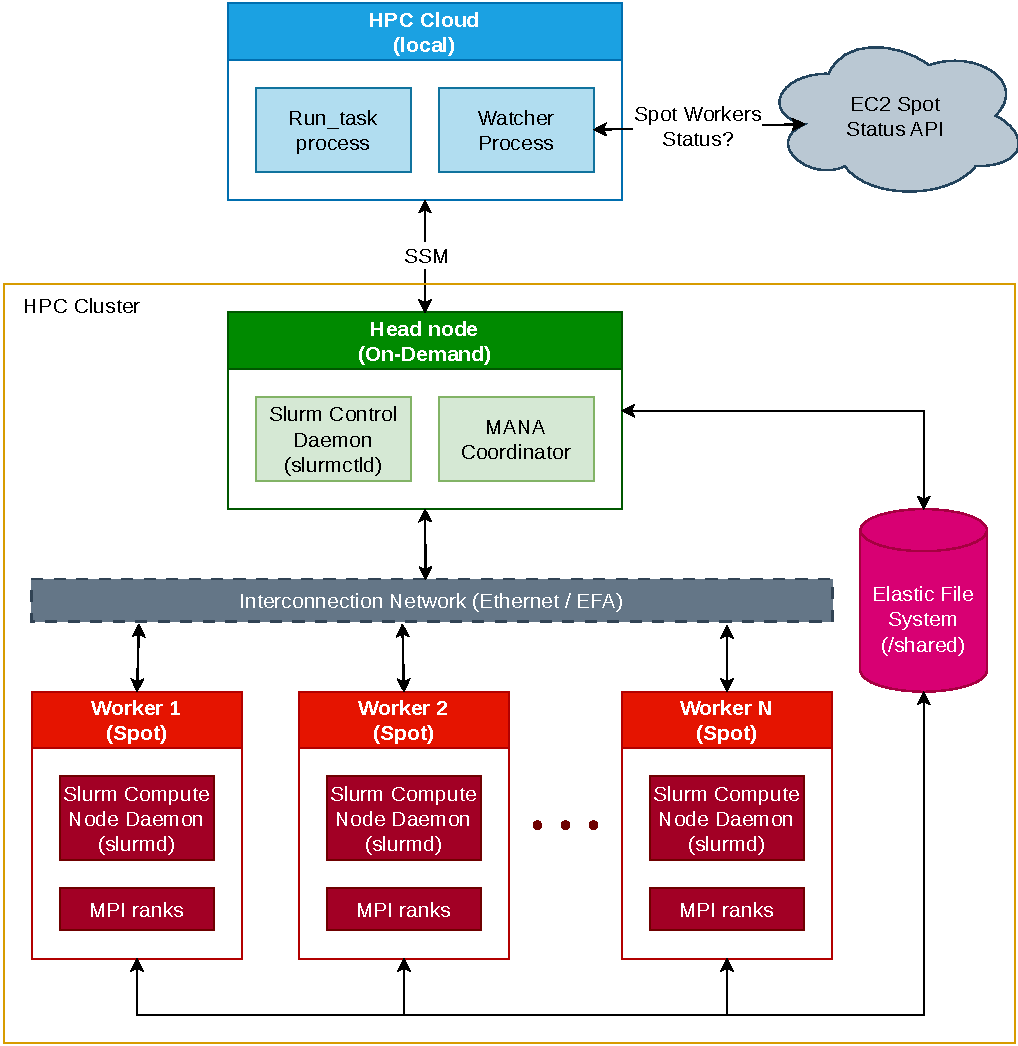
\includegraphics[width=\linewidth]{arch-overview-UCCversion}
        \end{column}
    \end{columns}
\end{frame}

%%%%%%%%%%%%%%%%%%%%%%%%%%%%
\showsections
\section{Estratégias de Recuperação}
%%%%%%%%%%%%%%%%%%%%%%%%%%%%

\begin{frame}{Duas Estratégias de Recuperação}
    O \textbf{Watcher} detecta o aviso, aciona o checkpoint e inicia uma das duas estratégias:
    \vspace{0.5em}
    \begin{itemize}
        \item \textbf{\textsc{Replace}:} provisiona um novo nó e restaura a capacidade original do \textit{cluster}
        \begin{itemize}
            \vspace{0.2em}
            \item Recuperação em $\approx$ 120\,s (aguarda nova instância)
            \item Retoma em capacidade total
        \end{itemize}
        \vspace{0.5em}
        \item \textbf{\textsc{Degraded}:} reinicia imediatamente nos nós sobreviventes
        \begin{itemize}
            \vspace{0.2em}
            \item Recuperação em $\approx$ 11\,s (reinício imediato)
            \item Retoma com paralelismo reduzido
        \end{itemize}
    \end{itemize}
    \vspace{0.6em}
    \small\textsc{Replace} garante capacidade total, mas exige mais tempo de recuperação. \textsc{Degraded} recupera imediatamente, porém com menor paralelismo.
\end{frame}

%%%%%%%%%%%%%%%%%%%%%%%%%%%%
\showsections
\section{Avaliação Experimental}
%%%%%%%%%%%%%%%%%%%%%%%%%%%%

\begin{frame}{Configuração Experimental}
    \begin{columns}
        \begin{column}{0.48\textwidth}
            \textbf{Ambiente (AWS):}
            \begin{itemize}
                \item \textit{Head}: t3.large (\textit{on-demand})
                \item \textit{Workers}: m5.xlarge (\textit{spot})
                \item \textit{Clusters} de \textbf{2, 4 e 8} \textit{workers}
            \end{itemize}
            \vspace{0.6em}
            \textbf{Experimentos:}
            \begin{itemize}
                \item Interrupções aos \textbf{10\%, 25\% e 50\%} da execução
                \item \textbf{282 execuções} no total
            \end{itemize}
        \end{column}
        \begin{column}{0.48\textwidth}
            \textbf{Benchmarks (NPB):}
            \begin{itemize}
                \item \textbf{EP-D:} comunicação mínima
                \item \textbf{CG-C:} comunicação intensa e irregular
                \item \textbf{LU-C:} comunicação estruturada
            \end{itemize}
            \vspace{0.6em}
            \small Três perfis distintos de comunicação MPI para avaliar o sistema em diferentes cenários
        \end{column}
    \end{columns}
\end{frame}

\begin{frame}{Comparação das Estratégias}
    \begin{columns}
        \begin{column}{0.52\textwidth}
            \centering
            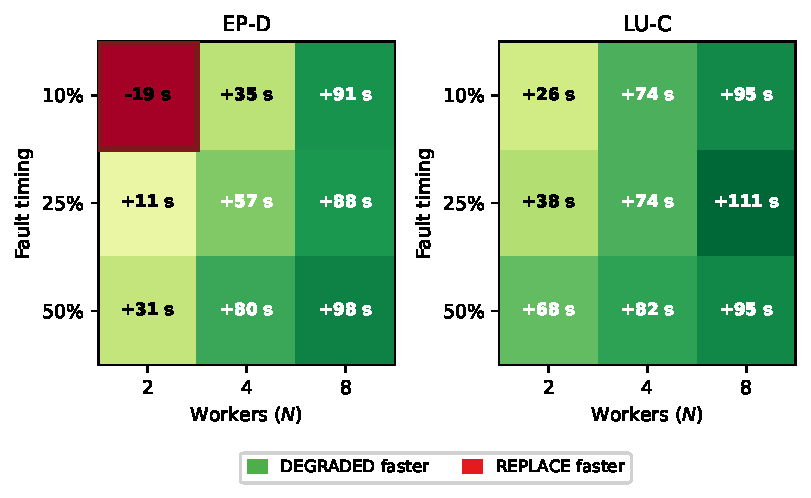
\includegraphics[width=\linewidth]{fig_crossover}
        \end{column}
        \begin{column}{0.45\textwidth}
            \small
            \textcolor{green!60!black}{\textbf{Verde}}: \textsc{Degraded} mais rápida \quad \textcolor{red!70!black}{\textbf{Vermelho}}: \textsc{Replace} mais rápida
            \vspace{0.5em}

            Dois fatores determinam a escolha:
            \begin{itemize}
                \vspace{0.2em}
                \item \textbf{Tamanho do cluster:} mais \textit{workers} $\Rightarrow$ menor impacto de perder um nó no \textsc{Degraded}
                \vspace{0.3em}
                \item \textbf{Momento da falha:} falha tardia $\Rightarrow$ pouco trabalho restante $\Rightarrow$ recuperação rápida compensa
            \end{itemize}
            \vspace{0.5em}
            Menor N + falha precoce $\Rightarrow$ menos verde (\textsc{Replace} vantajoso)\\
            Maior N + falha tardia $\Rightarrow$ mais verde (\textsc{Degraded} vantajoso)
        \end{column}
    \end{columns}
\end{frame}

\begin{frame}{Análise Econômica}
    \begin{columns}
        \begin{column}{0.62\textwidth}
            \centering
            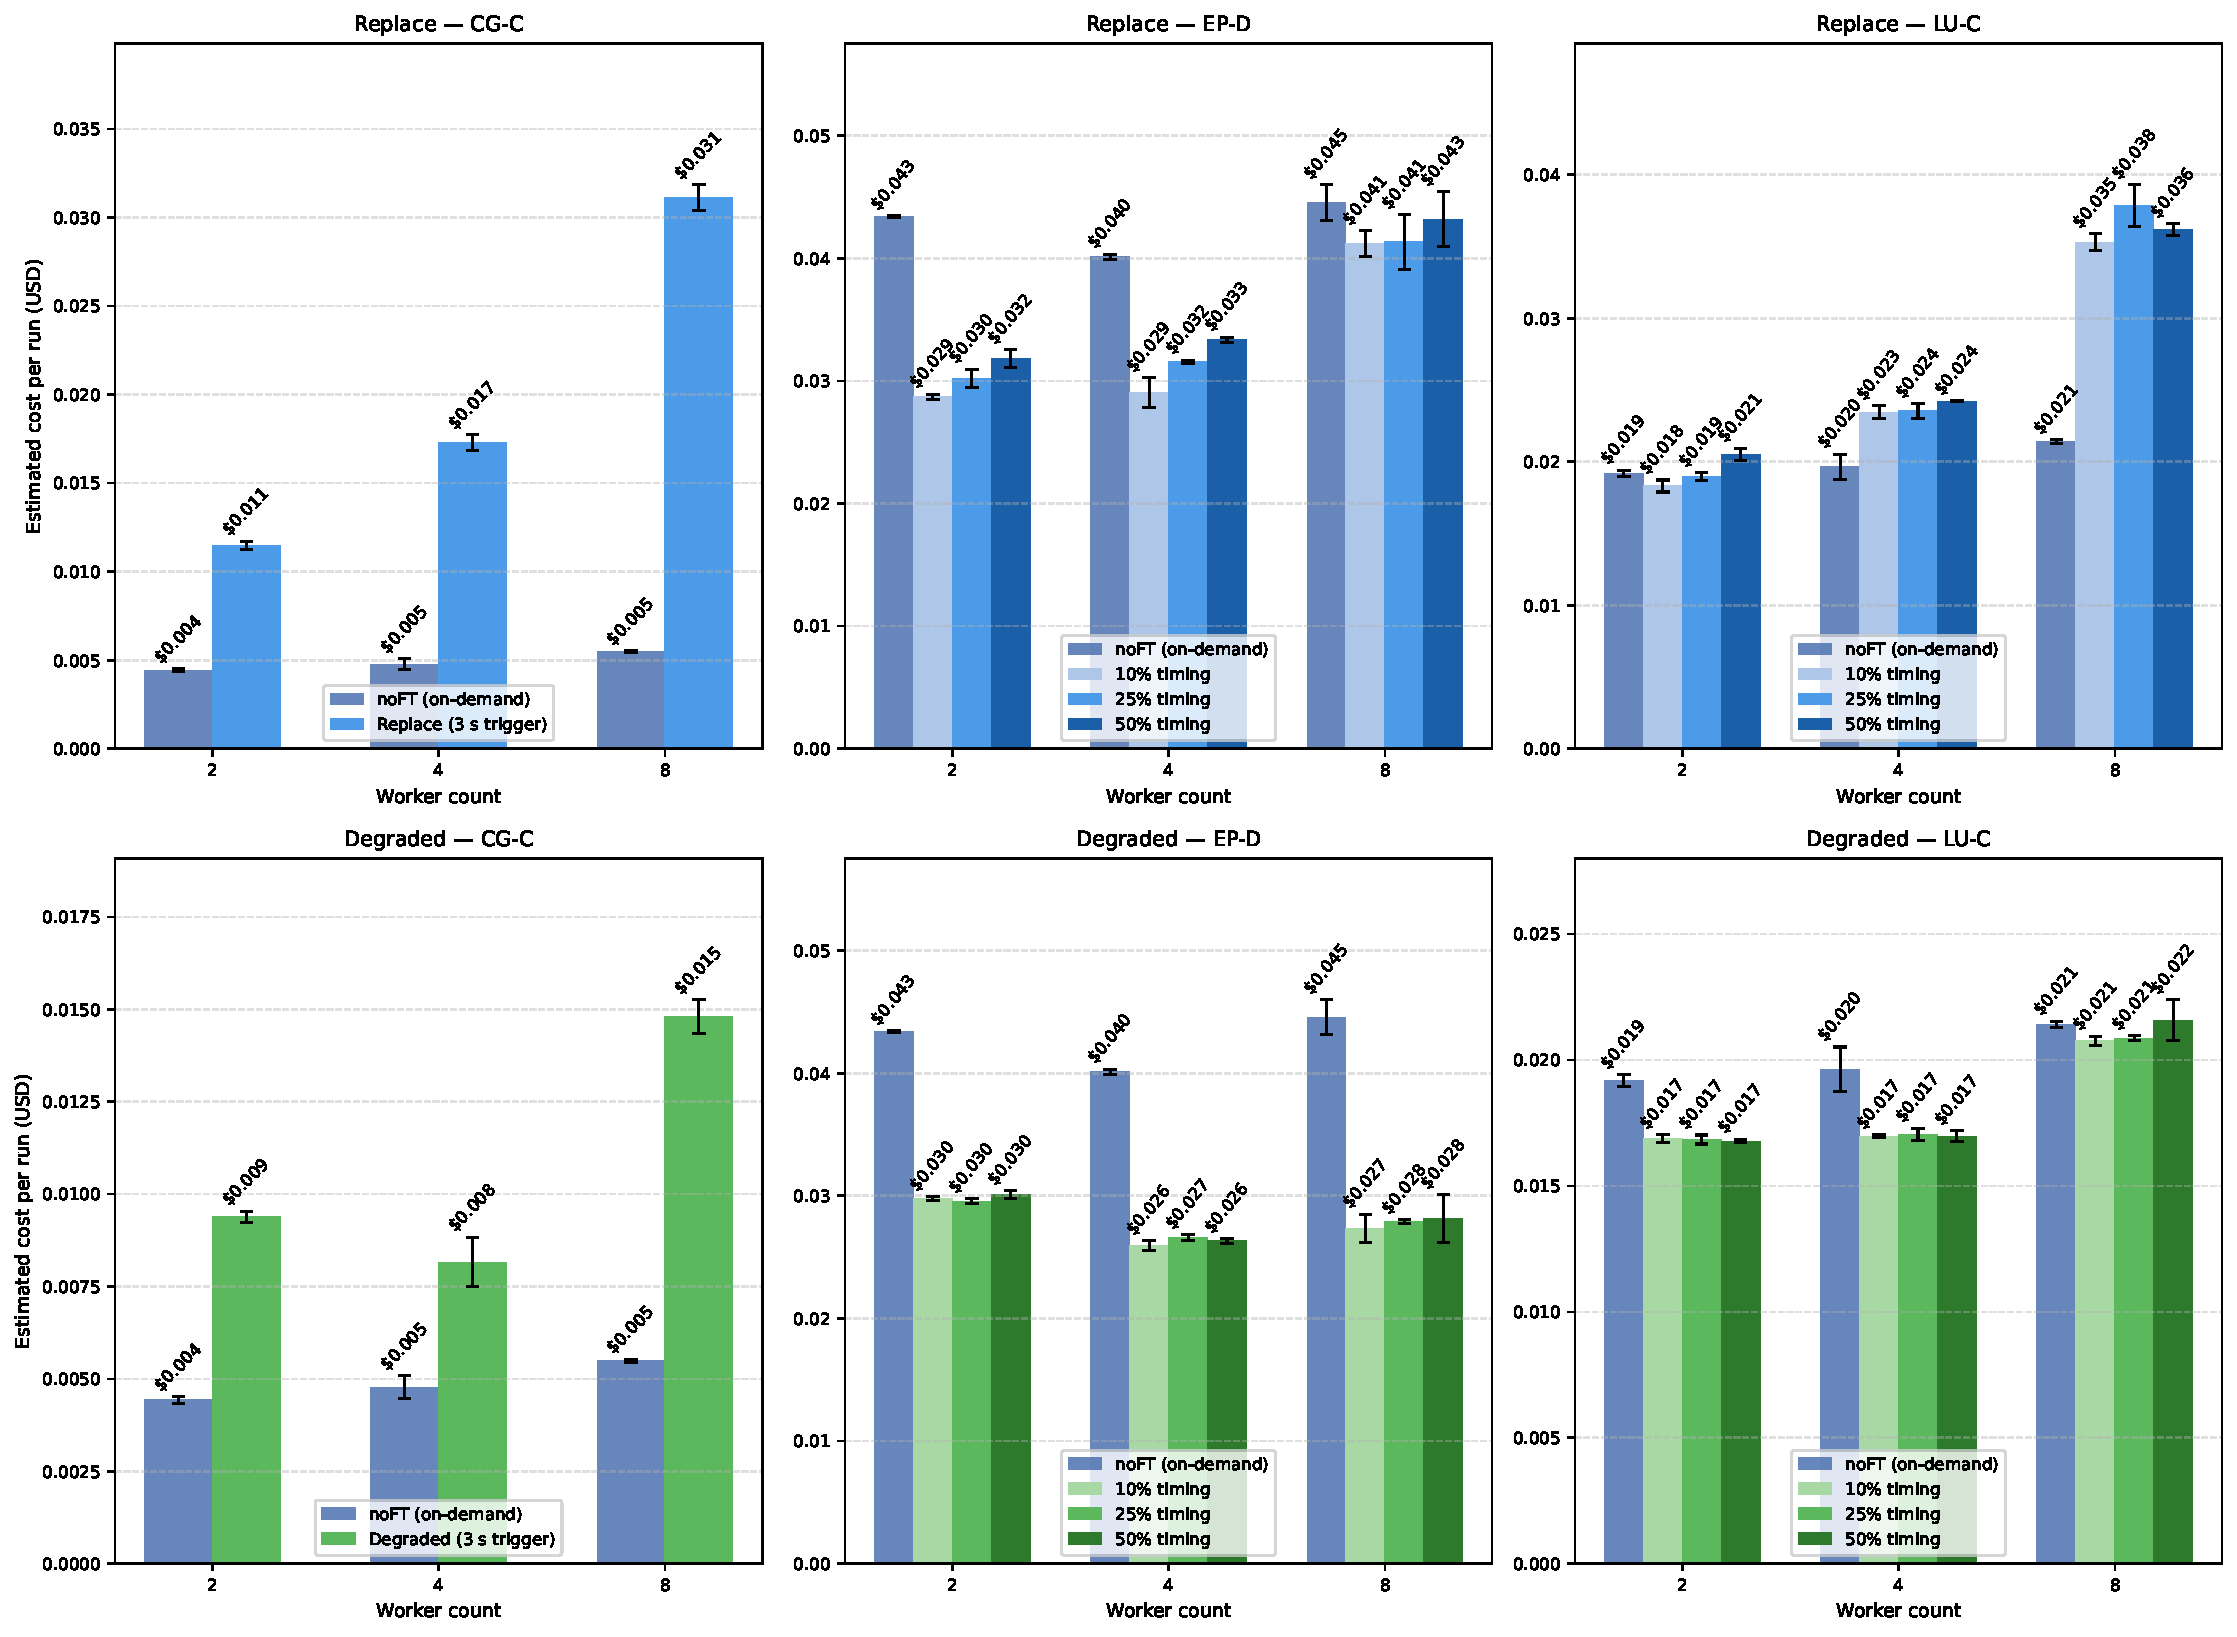
\includegraphics[width=\linewidth]{fig_cost}
        \end{column}
        \begin{column}{0.35\textwidth}
            \small
            O custo de recuperação é fixo; quanto mais longo o \textit{job}, menor seu impacto relativo:
            \vspace{0.4em}
            \begin{itemize}
                \item \textbf{EP-D} (longo): ambas as estratégias reduzem o custo total
                \vspace{0.2em}
                \item \textbf{LU-C} (médio): apenas \textsc{Degraded} é viável
                \vspace{0.2em}
                \item \textbf{CG-C} (curto): nenhuma estratégia reduz o custo
            \end{itemize}
            \vspace{0.4em}
            \textbf{A solução é viável e mais vantajosa em execuções de longa duração}
        \end{column}
    \end{columns}
\end{frame}

%%%%%%%%%%%%%%%%%%%%%%%%%%%%
\showsections
\section{Conclusão}
%%%%%%%%%%%%%%%%%%%%%%%%%%%%

\begin{frame}{Conclusão}
    \begin{itemize}
        \item Módulo de tolerância a falhas integrado ao HPC@Cloud com \textit{checkpoint} transparente para aplicações MPI
        \vspace{0.6em}
        \item Recuperação automática via \textsc{Replace} e \textsc{Degraded}, sem modificar o código da aplicação
        \vspace{0.6em}
        \item Solução viável economicamente para execuções de duração moderada a longa
        \vspace{0.6em}
        \item \textbf{Eixo UFSC: Tecnologia e Inovação}
    \end{itemize}
\end{frame}

%%%%%%%%%%%%%%%%%%%%%%%%%%%%
% Finalização
%%%%%%%%%%%%%%%%%%%%%%%%%%%%

\thanksframe

\end{document}
